\documentclass[twoside,11pt]{article}

% Any additional packages needed should be included after jmlr2e.
% Note that jmlr2e.sty includes epsfig, amssymb, natbib and graphicx,
% and defines many common macros, such as 'proof' and 'example'.
%
% It also sets the bibliographystyle to plainnat; for more information on
% natbib citation styles, see the natbib documentation, a copy of which
% is archived at http://www.jmlr.org/format/natbib.pdf

\usepackage{jmlr2e} 
\usepackage[bb=px]{mathalfa}
\usepackage{hyperref}
\graphicspath{{images/}}

% Definitions of handy macros can go here

\newcommand{\dataset}{{\cal D}}
\newcommand{\fracpartial}[2]{\frac{\partial #1}{\partial  #2}}

% Heading arguments are {volume}{year}{pages}{submitted}{published}{author-full-names}

\jmlrheading{1}{2023}{1-14}{3/24/23}{Justin Huang}

% Short headings should be running head and authors last names

\ShortHeadings{Analysis of Different Generator Architectures for Generative Adversial Networks (GANs)}{Justin Huang}
\firstpageno{1}

\begin{document}

\title{Analysis of Different Generator Architectures for Generative Adversial Networks (GANs)}

\author{\name Justin Huang \email jch004@ucsd.edu \\
    %    \addr Department of Statistics\\
       University of California, San Diego\\
       La Jolla, CA 92037, USA
}
\editor{Justin Huang}

\maketitle

\begin{abstract}%   <- trailing '%' for backward compatibility of .sty file
This paper describes the experiments of creating Generator models in Generative Adversial Networks (GANs) using different architectures and hyperparameters in order to find a model that can generate the most realistic images from random noise. Different methods such as Deep Convolutional layers, Conditional inputs, and Residual blocks are experimented, and the results are compared by looking at generator/discriminator loss and the quality of the generated images. The results show that a simple generator model with deep convolutional layers outperforms other models with conditional inputs and residual layers. Although the use of convolutional layers and the increase in parameters can help improve image quality and generation performance, increasing the complexity (as seen with residual layers) does not necessarily lead to better results. The analysis of different generator architectures in GANs can help the field of image generation understand the tradeoff between model complexity and performance.
\end{abstract}

\begin{keywords}
  Generative Adversial Networks (GANs), Residual Networks (ResNets), Image Synthesis/Generation
\end{keywords}

\section{Introduction}

As the world of deep learning continues to grow, newer applications of machine learning also continue to emerge. One of these recent applications is image generation, which is the process of generating images from random noise. For example, if you were to describe a picture of a flower to someone, they would be able to visualize the image in their head. To be able to correlate the relationship between numbers and visually realistic images is a big step for machines to match the human intellectual ability of creating new art. 

We have already seen the success of deep learning for image generation, with models such as DALL-E and Stable Diffusion training on millions of data. They both use diffusion models, which train by introducing Gaussian noise in training images in a series of timesteps, and learn to reverse this noising process. These models have outperformed previous generative models such as Generative Adversial Networks (GANs) in image synthesis.

However, despite the emergence of diffusion models, GANs can still prove to be an effective model for image synthesis. A simple GAN consists of two neural networks: a convolutional neural network to generate new data (the generator, \textbf{G}) and a neural network to classify real and generated data (the discriminator, \textbf{D}) \citet{brownlee:19}. The concept of GANs come from game theory, where we train the generator (G) to fool the discriminator (D) into being unable to distinguish between real and generated data. In other words, we want to minimize the loss function of the discriminator and maximize the loss function of the generator.

We can also add onto the basic idea of GANs by generating images based on a class label input, or by changing the architecture of the generator/discriminator with convolutional layers or residual blocks.

In this paper, I will train a GAN with various generator architectures and hyperparameters on the CIFAR-10 dataset, and compare the results to see which generator model is the most effective in generating realistic 64x64 RGB images. I will incorporate ideas from Deep Convolutional GANs (DCGAN), conditional Deep Convolutional GANs (cDCGAN), and Residual Convolutional GANs (RC-GAN) to see which combination can generate the best images from random noise and the class label. The model performance will be evaluated by the loss and the quality of the generated images.

\section{Related Work}

The idea of using both generative and discriminative models \citet{goodfellow:14} has been around for awhile, but the initial implementations resulted in noisy and unrealistic images. Still, even with such a basic architecture as multi-layer perceptrons, the unique concept of GANs based off game theory has revolutionalized future generative models that also didn't need Markov chains anymore.

In order to add more information for the generator and discriminator models to learn from, conditional GANs (cGANs) were introduced \citet{mirza:14}. cGANs feed in both random noise and a class label of the image to be generated, which allows the generator to create images based on the class label, and the discriminator to be able to distinguish between the different classes.

Later, convolutional (and tranposed convolutional) layers were introduced into the GAN architecture \citet{radford:16}, otherwise known as Deep Convolutional GANs (DCGAN). Since convolutional layers are good at extracting features from images, it made sense that more realistic images could be generated. In this implementation, the generator would take in random noise and upsample (transpose convolutional layers) to the desired image size, and the discriminator would take in the generated image and downsample (convolutional layers) to a single value.

Furthermore, \citet{hyland:17} has shown that residual blocks can be added to the generator and discriminator to experiment with the performance of the model. Residual blocks are a type of convolutional layer that can be stacked on top of each other, and they allow the model to learn more complex features with extra "skip connections." In theory, adding more complex connections between layers can help the model learn more complex features, and therefore generate more realistic images. However, \citet{he:21} and his experiments have shown that Resnet generator architectures sometimes underperform compared to regular CNN architectures.

We will use the cumulation of these ideas to experiment and create an optimal generator model for a Deep Convolutional GAN (DC-GAN).

\section{Dataset}

I will be using the CIFAR-10 training dataset, which consists of 50,000 32x32 RGB images of 10 different classes: airplane, automobile, bird, cat, deer, dog, frog, horse, ship, and truck. The images are all normalized to be between 0 and 1, and class labels are integers from 0 to 9. Testing will be done on a fixed batch of latent vectors with their corresponding (random) class labels to assess the quality of generated images across models.

\section{Method/Architecture}

I will build three different architectures of the Generator model for GANs: a regular DC-GAN with convolutional layers, a conditional DC-GAN that adds the class label as input, and a residual conditional DC-GAN that adds residual blocks into the architecture. When testing all three architectures, the discriminator model will be kept the same. 

I will use the following discriminator model from \citet{radford:16} (as seen in Figure \ref{fig:discriminator}).

\begin{figure}[h!]
  \centering
  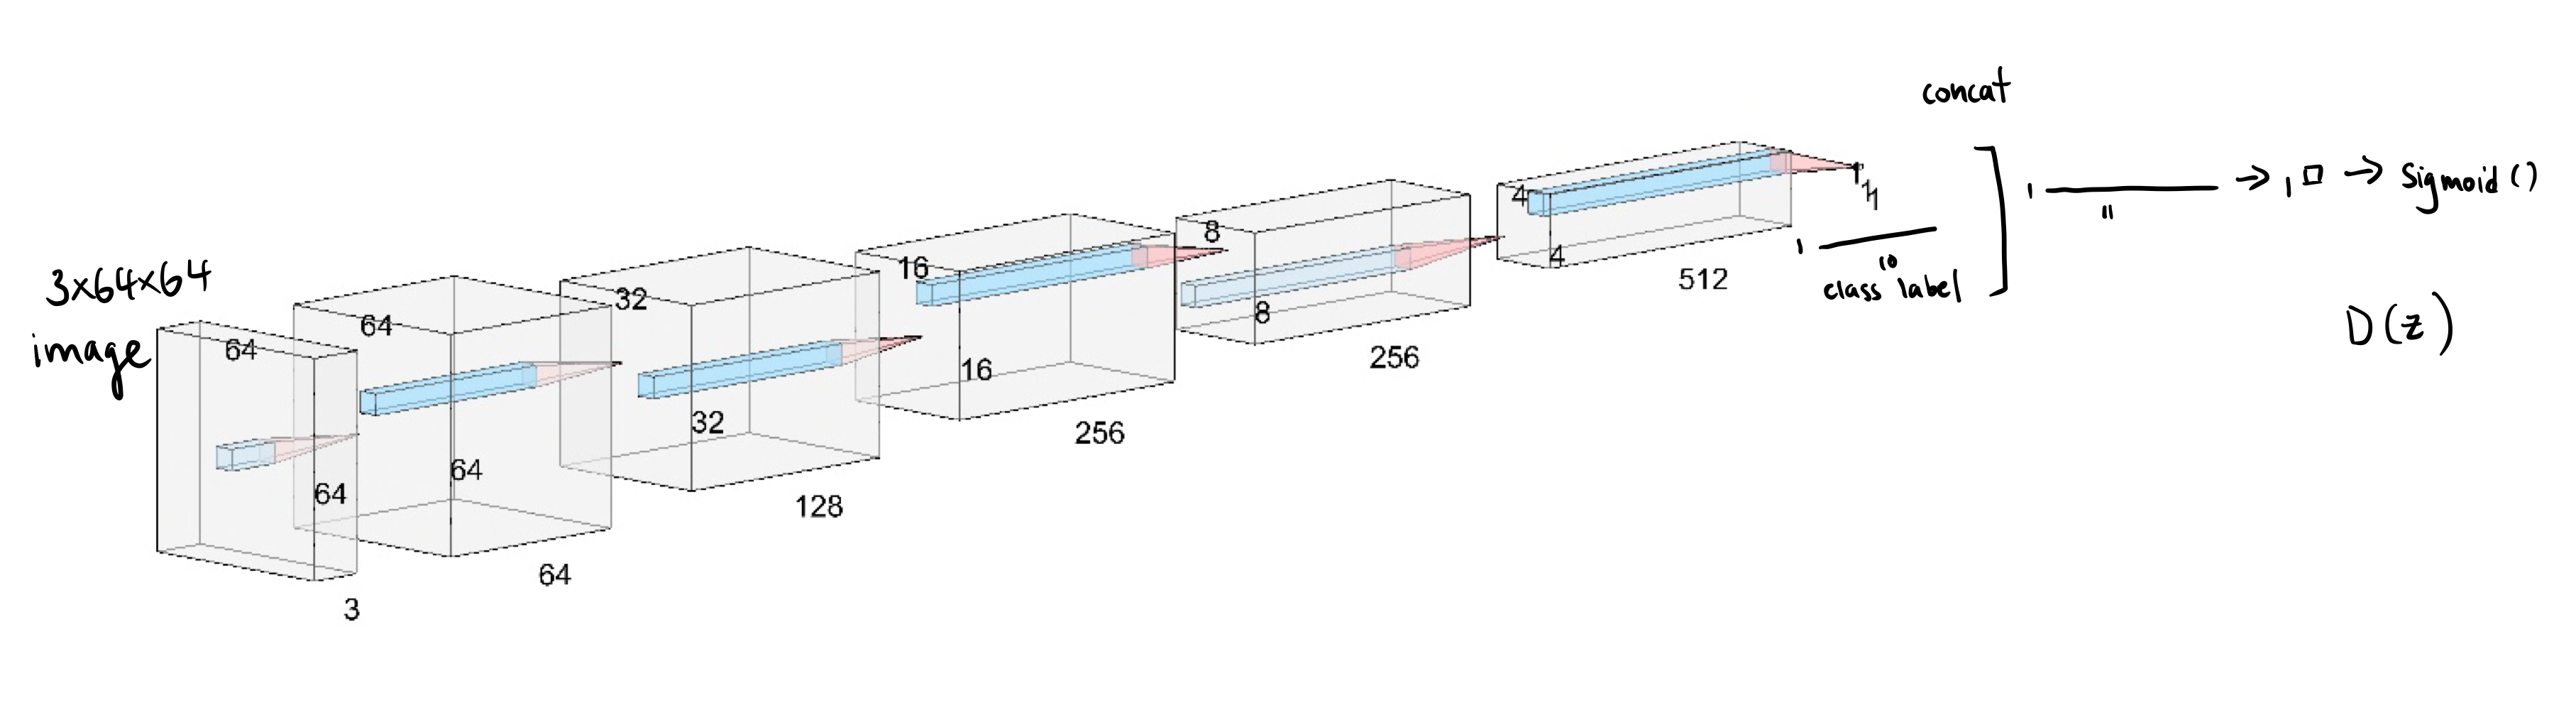
\includegraphics[width=\textwidth]{images/discriminator.png}
  \caption{Discriminator Model for GAN. A 64x64 RGB image is passed into the model, and downsampling is performed using convolutional layers to generate a single value. For simple DC-GANs, the architecture stops here. For DC-GANs with conditional inputs, the output is then concatenated with one-hot encoded class label and fed through a linear layer to generate another single value that determines if an image is real or fake.}
  \label{fig:discriminator}
\end{figure}

\begin{figure}[h!]
  \centering
  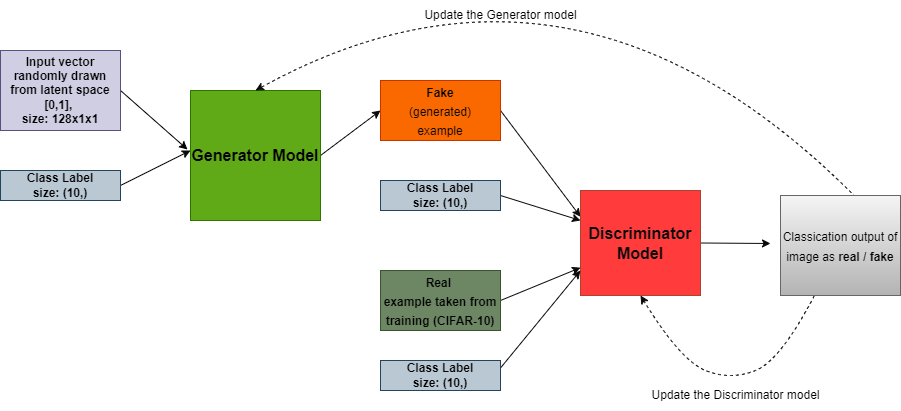
\includegraphics[width=\textwidth]{images/gan.png}
  \caption{General Architecture for Conditional GANs. For simple DC-GANs, we just pass in the random noise vector into the generator model, and the fake/real image into the discriminator model.}
  \label{fig:dcgan-3}
\end{figure}

\noindent I also followed the guidelines found by \citet{radford:16} for stable Deep Convolutional GANs:

\begin{itemize}
  \item Replace any pooling layers with strided convolutions (discriminator) and fractional-strided convolutions (generator).
  \item Use batchnorm in both the generator and the discriminator.
  \item Use ReLU activation in generator for all layers except for the output, which uses Tanh.
  \item Use LeakyReLU activation in the discriminator for all layers.
\end{itemize}

\newpage

\section{Experiment Setup}
% ( data and problem description, hyper-parameters, training process etc.)

\subsection{Problem Description}

The goal of this paper is to test different generator architectures for the GAN on the CIFAR-10 dataset, and compare the results to find the architecture that generates the most realistic images. I will build 3 models that will progressively be optimized: a DC-GAN, a conditional DC-GAN (DC-cGAN), and finally the residual conditional GAN (RC-cGAN). During the training of each model, I will experiment with different hyperparameters, activation functions, and number of filters/layers. The model performance will be evaluated on the loss function of both the discriminator/generator. In addition, I will also use a constant batch of 64 latent vectors of length 128 (and their corresponding constant class labels) to track the progress of image synethesis. The quality of these generated images will then be used to evalulate/compare the success of the models.

\subsection{Pre-Processing Data}

The CIFAR-10 dataset has already normalized the images to the range [0, 1], and all images are 32x32 RGB images. For all models built, we have applied the following pre-processing steps: 

\begin{enumerate}
  \item Resizing the images to 64x64 RGB images
  \item Crop the 64x64 RGB images to the center
  \item Normalize the images with means [0.5, 0.5, 0.5] and standard deviations [0.5, 0.5, 0.5]
\end{enumerate}

\subsection{Loss Function and Optimizer}

For all the models, I've decided to keep the loss function and optimizer the same. I will use the \textbf{Binary Cross Entropy Loss (BCELoss)} for my loss function, and the \textbf{Adam Optimizer} for my optimizer. The betas will be set to (0.5, 0.999).

To maximize the loss function D(z), we will use the BCELoss function with the real images as the target, and the fake images as the input. To maximize the loss function D(G(z)), we will use the BCELoss function with the fake images as the target, and the output of the discriminator as the input. To minimize the loss function G(z), we will use the BCELoss function with the fake images as the target, and the output of the discriminator as the input.

$$\min_{\theta_g}\max_{\theta_d}[\mathbb{E}_{x\sim p_{data}}\log D_{\theta_d}(x) + \mathbb{E}_{z\sim p(x)} \log(1-D_{\theta_d}(G_{\theta_g}(z)))]$$

\textbf{Note:} I did try some experiments with using Stochastic Gradient Descent (SGD) as the optimizer, but the discriminator loss always zeroed out after a few epochs (meaning the discriminator was really good at differentiating fake and real images). 

\subsection{Hyperparameters}

The hyperparameters that I will be tuning for each model are the following:

\begin{itemize}
  \item \textbf{Batch Size}: 32, 64, 128
  \item \textbf{Number of Epochs}: 30, 50, 80
  \item \textbf{Learning Rate}: 0.001
  \item \textbf{Latent Vector Size}: 128
\end{itemize}

\section{Experiment}

\subsection{Deep Convolutional GAN (DC-GAN)}

In my experiments, I started with \citet{radford:16}'s optimal model, and fine-tuned with different numbers of filters and convolutional layers (Figure \ref{fig:dcgan-archs}). For the basic GAN with convolutional layers, I found the best architecture to have 6 upsampling convolutional layers, and 1 downsampling convolutional layer, with 2 times more filters for each layer compared to \citet{radford:16} (Figure \ref{fig:best-dcgan}). 

\begin{figure}[h!]
  \centering
  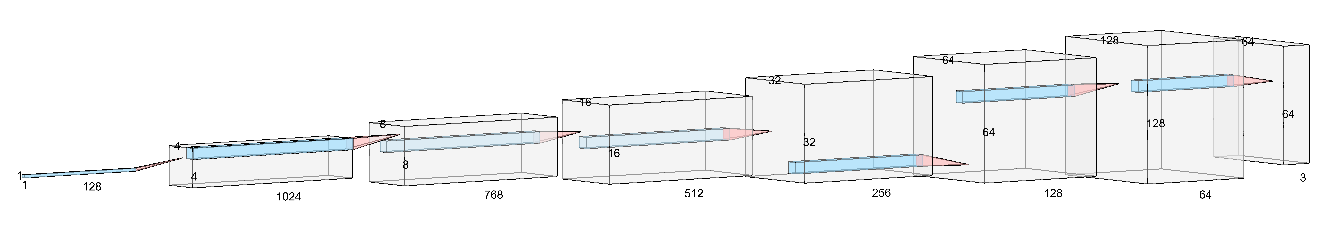
\includegraphics[width=17cm]{images/dcgan-experiments/dcgan4.png}
  \caption{\textbf{Best} Generator Model for GAN with deep convolutional layers (DC-GAN).}
  \label{fig:best-dcgan}
\end{figure}

\begin{figure}[h!]
  \centering
  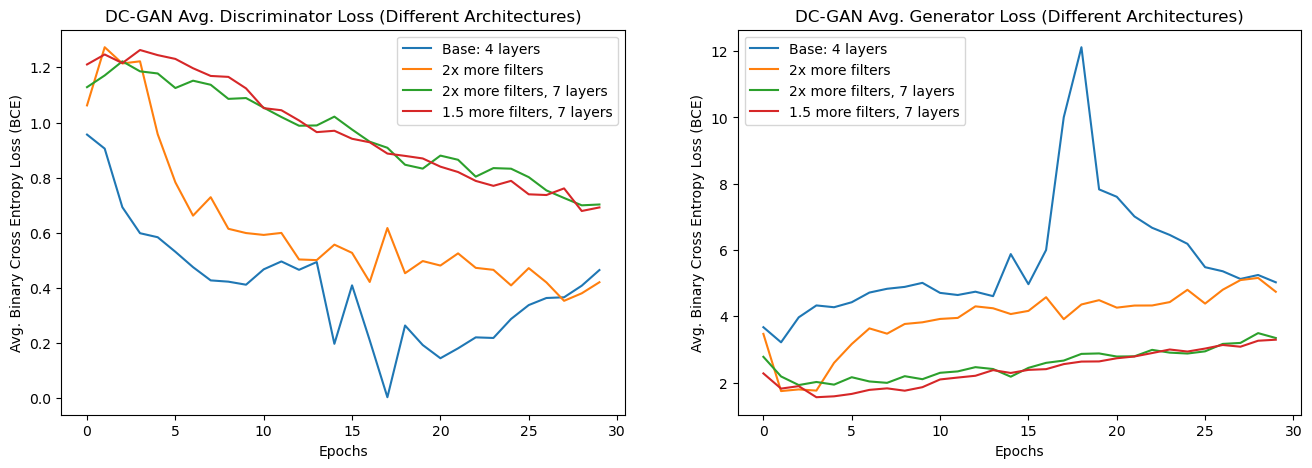
\includegraphics[width=16cm]{images/dcgan-experiments/dcgan-archs.png}
  \caption{Discriminator and Generator losses with different architectures for DC-GAN.}
  \label{fig:dcgan-archs}
\end{figure}

I ended up using \textbf{ReLU as the primary activation function} for all layers except the last, which used Tanh. In my experiments (Figure \ref{fig:dcgan-activations}), GELU actually had lower loss for the generator than ReLU when the epochs were low ($<$ 30). However, as the epochs increased, the generated images started to look more like noise, while the ReLU images started to look more realistic. 

\begin{figure}[h!]
  \centering
  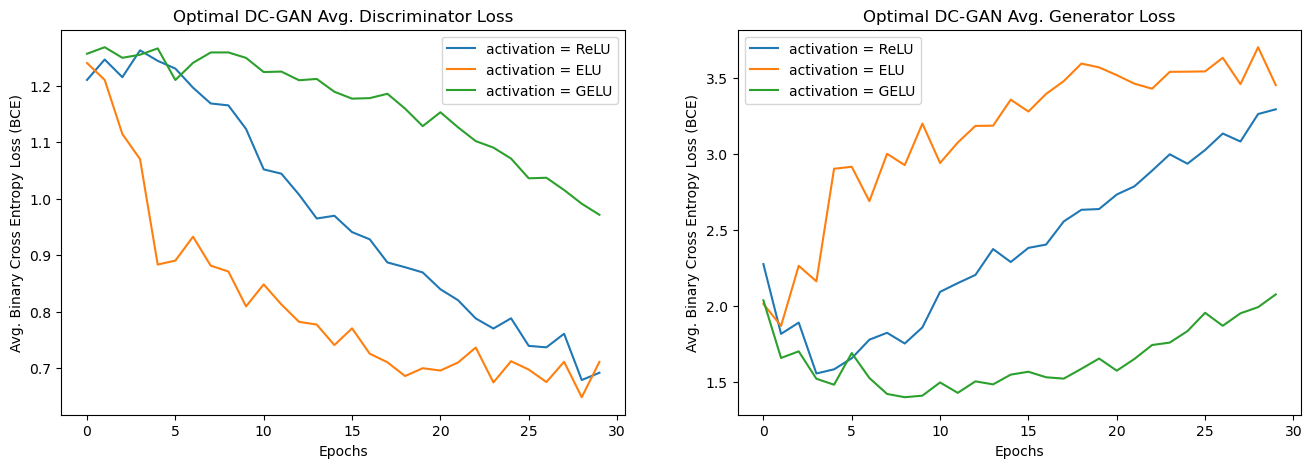
\includegraphics[width=16cm]{images/dcgan-experiments/dcgan-activations.png}
  \caption{Discriminator and Generator losses with different activation functions for DC-GAN.}
  \label{fig:dcgan-activations}
\end{figure}

Lastly, I experimented with batch sizes of 32, 64, and 128, and found the best results with a \textbf{batch size of 128} (Figure \ref{fig:dcgan-batchsizes}).

\begin{figure}[h!]
  \centering
  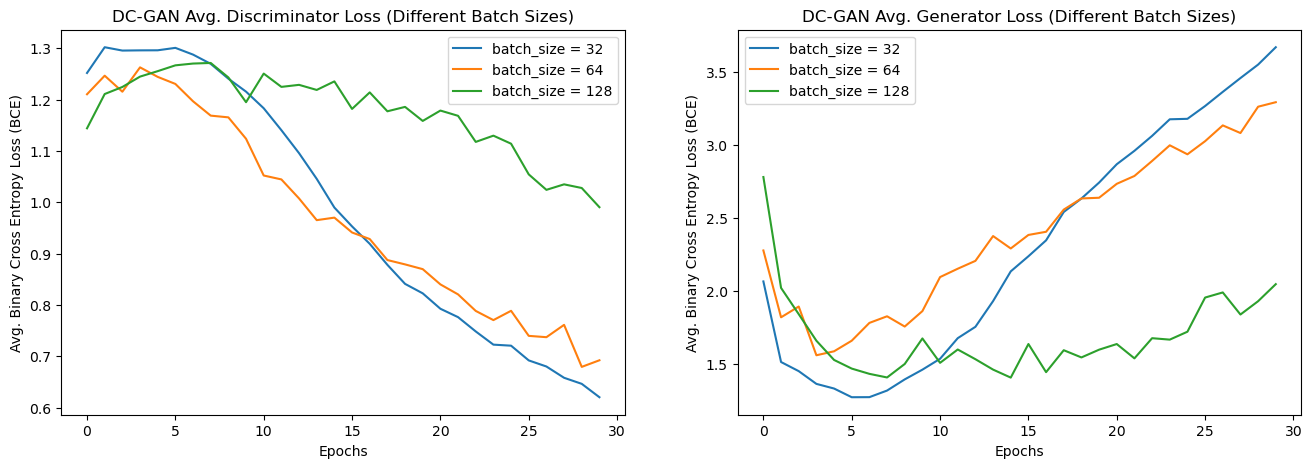
\includegraphics[width=16cm]{images/dcgan-experiments/dcgan-batchsizes.png}
  \caption{Discriminator and Generator losses with different batch sizes for DC-GAN.}
  \label{fig:dcgan-batchsizes}
\end{figure}

\newpage

\noindent In the end, the hyperparameters that I used for the DC-GAN were the following:

\begin{itemize}
  \item \textbf{Batch Size}: 128
  \item \textbf{Number of Epochs}: 30
  \item \textbf{Learning Rate}: 0.001
  \item \textbf{Latent Vector Size}: 128
\end{itemize}

Some sample generated images over 30, 50, and 80 epochs with the optimal DC-GAN generator architecture are shown in Figure \ref{fig:dcgan-outputs}, but not much improvement is seen beyond 50 epochs.

\begin{figure}[h!]
  \centering
  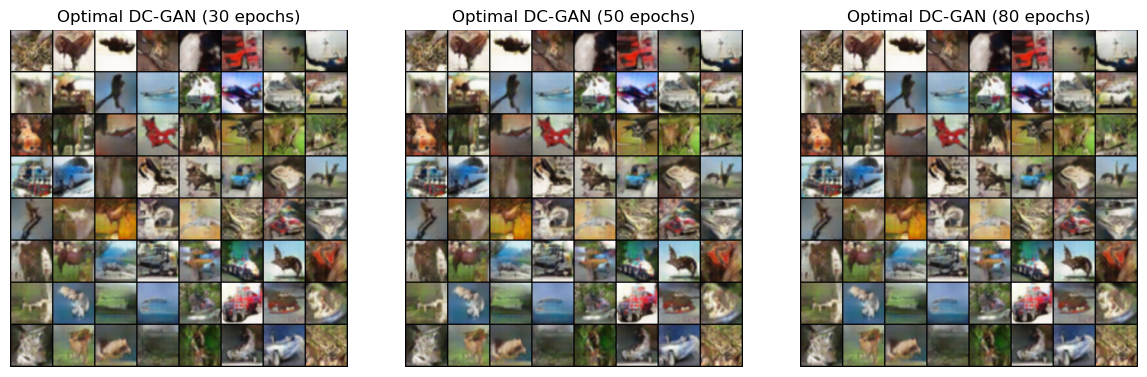
\includegraphics[width=18cm]{images/dcgan-experiments/dcgan-outputs.png}
  \caption{Generated images from best DC-GAN model over 30, 50, and 80 epochs.}
  \label{fig:dcgan-outputs}
\end{figure}

\subsection{Conditional Deep Convolutional GAN (cDCGAN)}

Next, I experimented with adding a conditional input, which was the class label of the images, to both the generator and discriminator. This architecture is known as a conditional GAN (DC-cGAN), where we give the GAN a little more information about the images they are generating.

I found the best Deep Convolutional Conditional Generator architecture to have 6 upsampling convolutional layers and 1 downsampling layer, each with 2 times more filters than the previous layer (Figure \ref{fig:best-dccgan}, Figure \ref{fig:dccgan-archs}). I also experimented with adding Average Pooling and Dropout layers, but found that they worsened the generated images, and tended to minimized the loss of the discriminator (opposite of what we want!).

\begin{figure}[h!]
  \centering
  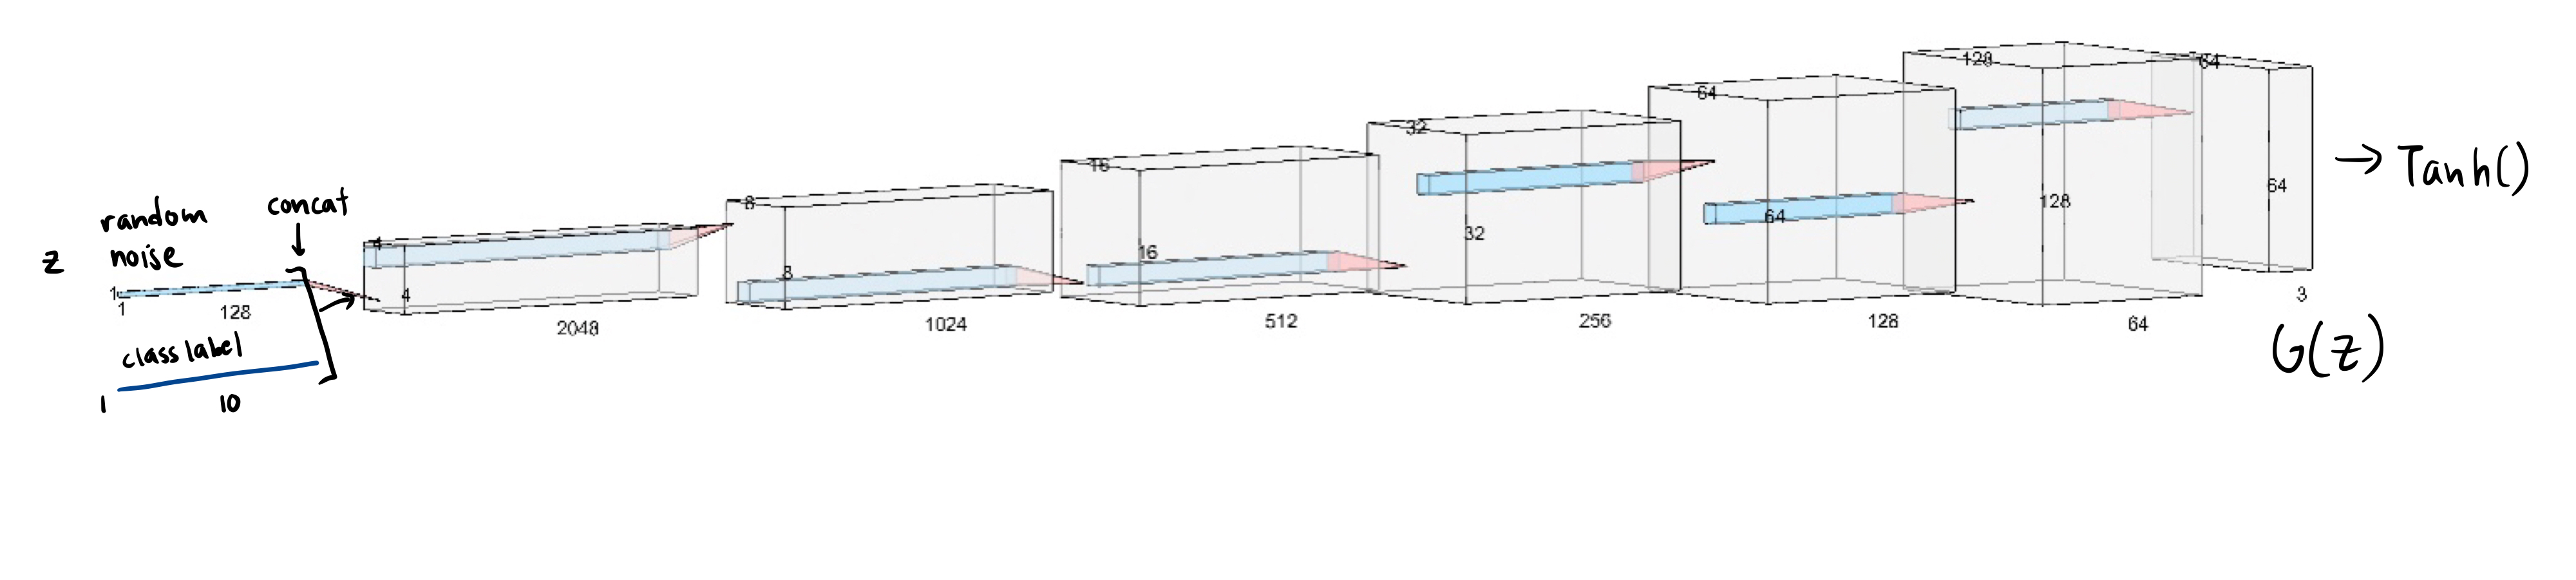
\includegraphics[width=18cm]{images/dccgan-experiments/dccgan8.jpeg}
  \caption{\textbf{Best} Generator Model for GAN with deep convolutional layers and conditional input (DC-cGAN).}
  \label{fig:best-dccgan}
\end{figure}

\begin{figure}[h!]
  \centering
  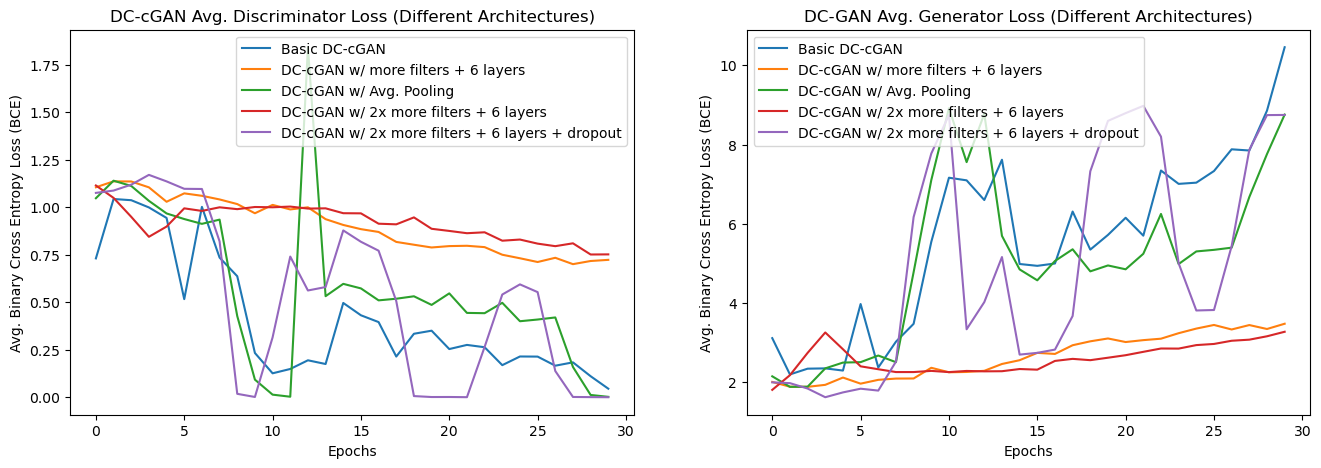
\includegraphics[width=17cm]{images/dccgan-experiments/dccgan-archs.png}
  \caption{Discriminator and Generator losses with different architectures for DC-cGAN.}
  \label{fig:dccgan-archs}
\end{figure}

I ended up using ReLU as the primary activation function with the DC-cGAN for the same reasons as the DC-GAN model: GELU had lower losses for the generator, but generated images were not as realistic as epochs increased (Figure \ref{fig:dccgan-activations}).

\begin{figure}[h!]
  \centering
  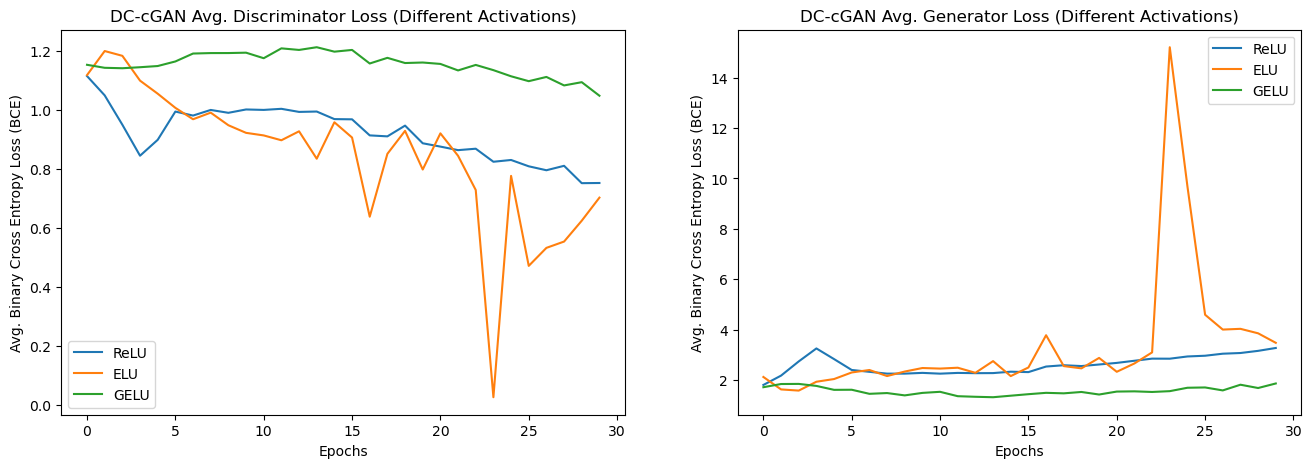
\includegraphics[width=16cm]{images/dccgan-experiments/dccgan-activations.png}
  \caption{Discriminator and Generator losses with different activation functions for DC-cGAN.}
  \label{fig:dccgan-activations}
\end{figure}

\newpage

Lastly, I experimented with the hyperparameters. I kept the batch size at 128, but played around with epochs of 30, 50, and 80 for this model. I found that the best results were with 80 epochs. Interestingly, the generated images improved as the epochs increased with the best DC-cGAN, compared to little-to-no improvement with DC-GAN. The generated images at the end of each epoch can be found in Figure \ref{fig:dccgan-outputs}.

\noindent In the end, the hyperparameters that I used for the DC-GAN were the following:

\begin{itemize}
  \item \textbf{Batch Size}: 128
  \item \textbf{Number of Epochs}: 50
  \item \textbf{Learning Rate}: 0.001
  \item \textbf{Latent Vector Size}: 128
\end{itemize}

\begin{figure}[h!]
  \centering
  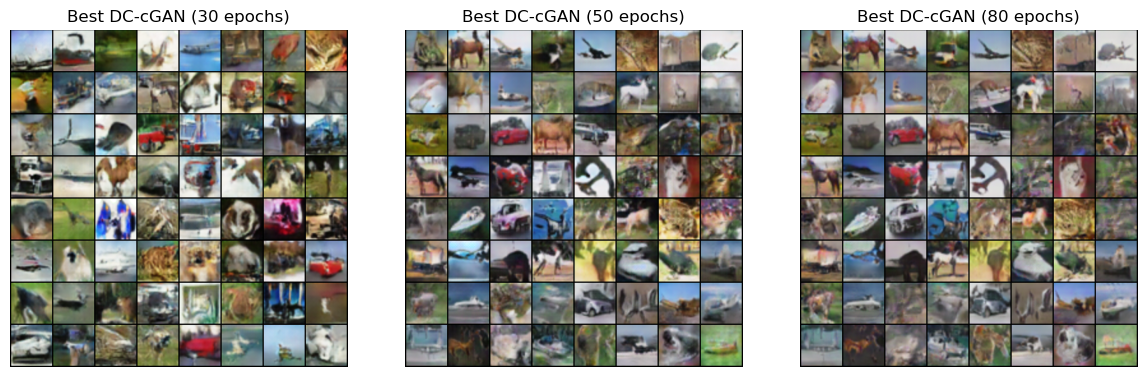
\includegraphics[width=16.5cm]{images/dccgan-experiments/dccgan-outputs.png}
  \caption{Generated images from best DC-GAN model over 30, 50, and 80 epochs.}
  \label{fig:dccgan-outputs}
\end{figure}

\newpage

\subsection{Residual Conditional Deep Convolutional GAN (RC-cGAN)}

I also experimented with using ResNet-18 and ResNet-34 architectures for the generator. Due to computational power limitations (training taking too long), I only modified the architecture. I implemented by replacing all the downsampling convolutional residual blocks with upsampling convolutional layers. I also removed the average pooling layer, and replaced the fully-connected layer with a single downsampling convolutional layer. Through my experiments, I found that ResNet-18 had a better generator loss than ResNet-34, and generated more realistic images (Figure \ref{fig:rccgan-outputs}). 

The hyperparameters that I used for the RC-cGAN were the following:

\begin{itemize}
  \item \textbf{Batch Size}: 128
  \item \textbf{Number of Epochs}: 30
  \item \textbf{Learning Rate}: 0.001
  \item \textbf{Latent Vector Size}: 128
\end{itemize}

\begin{figure}[h!]
  \centering
  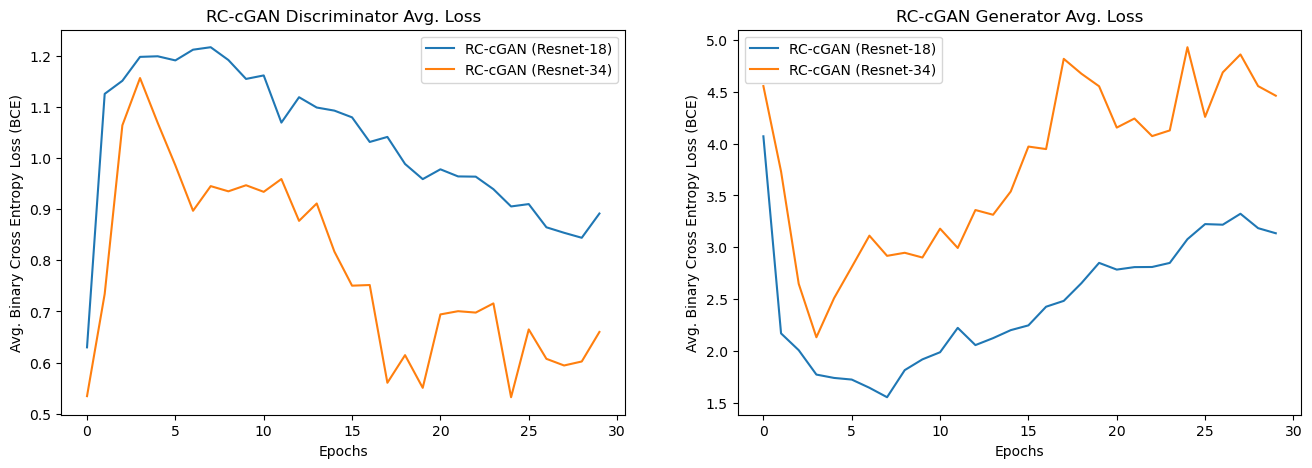
\includegraphics[width=16cm]{images/rccgan-experiments/rccgan-archs.png}
  \caption{Discriminator and Generator losses with different activation functions for DC-cGAN.}
  \label{fig:rccgan-archs}
\end{figure}

\begin{figure}[h!]
  \centering
  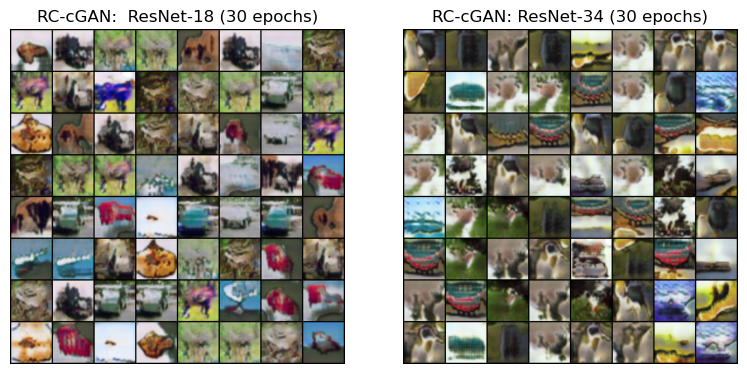
\includegraphics[width=15cm]{images/rccgan-experiments/rccgan-outputs.png}
  \caption{Generated images from RC-cGAN models with ResNet-18 and ResNet-34 architectures.}
  \label{fig:rccgan-outputs}
\end{figure}

\newpage

\subsection{Results Comparison}

Finally, I compared the results of the different generator architectures for the GAN to determine the best performing model. I first looked at the discriminator and generator losses. The model that maximized the discriminator losses and minimized the generator losses the most was actually the simple GAN with deep convolutional layers (DC-GAN), as seen in Figure \ref{fig:results-losses}.

\begin{figure}[h!]
  \centering
  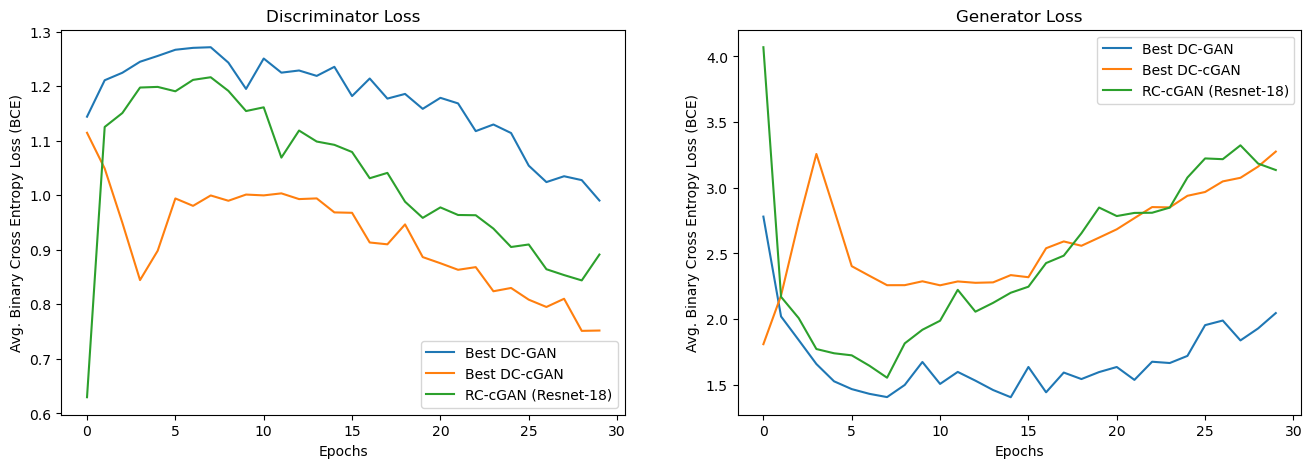
\includegraphics[width=16cm]{images/results-losses.png}
  \caption{Generator and Discriminator losses from the best models of each GAN architecture}
  \label{fig:results-losses}
\end{figure}

I also compared the "real" and "generated" scores of each generator model, where the score is the average of the discriminator's classification output for a given image (0 is generated, 1 is real). We want the "real score" to be closer to 0.5, and the "generated score" to be closer to 1. Again, the simple DC-GAN model had the best generated scores (generated images were getting classified as real more often), as seen in Figure \ref{fig:results-scores}.

\begin{figure}[h!]
  \centering
  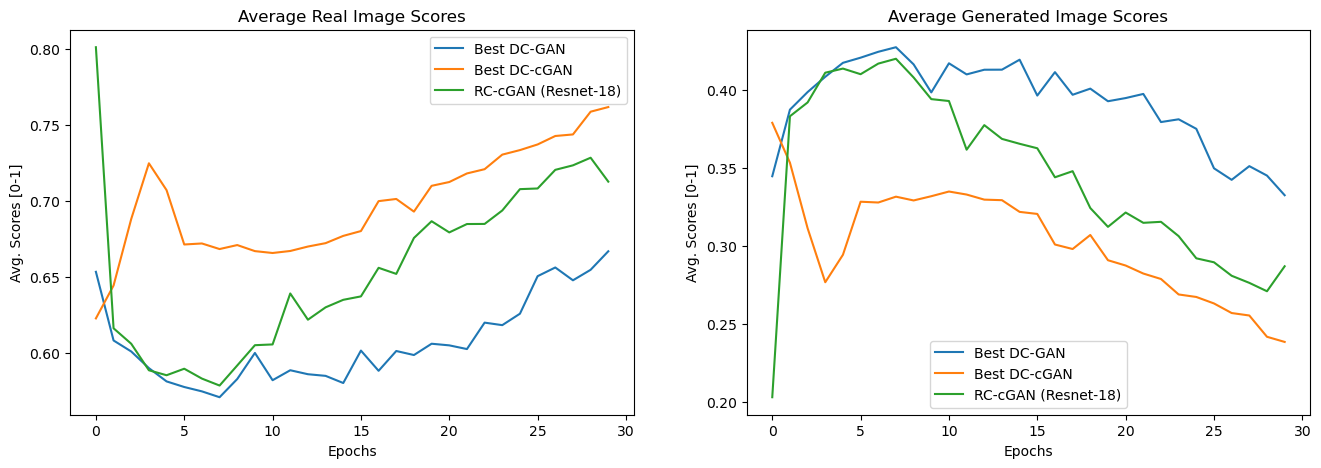
\includegraphics[width=16cm]{images/results-scores.png}
  \caption{Generator and Discriminator real and generated scores from the best models of each GAN architecture}
  \label{fig:results-scores}
\end{figure}

Looking at the generated images at 50 epochs, we can see that the DC-GAN and the DC-cGAN models generated realistic images for some latent vector inputs, as seen in Figure \ref{fig:results-outputs}. The RC-cGAN also had some good generated images of planes, but had problems with everything else. Subjectively, I found the DC-cGAN to generate better images, the DC-GAN to be a close second, and the RC-cGAN to be the worst.

\begin{figure}[h!]
  \centering
  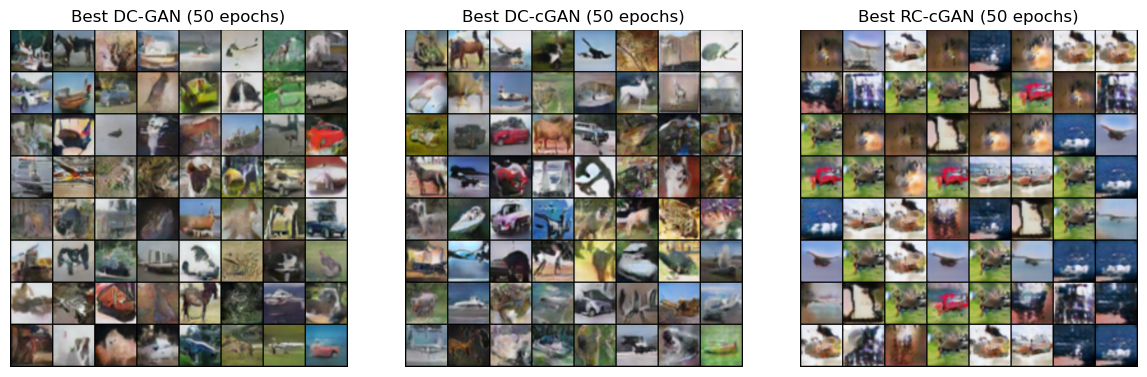
\includegraphics[width=18cm]{images/results-outputs-small.png}
  \caption{Generated Images from the best }
  \label{fig:results-outputs}
\end{figure}

\newpage

\section{Conclusion}

In this report, I built different generator architectures for GANs and analyzed their performance for image generation. I experimented with a deep convolutional GAN (DC-GAN), a deep convolutional GAN with conditional inputs (DC-cGAN), and a deep convolutional GAN with residual layers and conditional inputs (RC-cGAN). For each architecture, I also trialed different activation functions and hyperparameters. I found that the simple DC-GAN was the best model that maximized the discriminator loss, minimized the generator loss, and still generated (mostly) realistic images. The RC-cGAN had the worst discriminator and generator losses, and generated images that were not as realistic as the DC-GAN. As I experimented each architecture, I also found that increasing the number of parameters did help with improving model performance and image quality.

The results illustrate that increasing the complexity of the generator architecture, as seen with the RC-cGAN experiments, does not necessarily lead to better results. Using deep convolutional layers and increasing the number of parameters, however, have still proven to be effective in improving the performance of GANs. These results may be used to inform future design choices for generator architectures in GANs, and to trial with different datasets.

% Acknowledgements should go at the end, before appendices and references

\acks{I would like to acknowledge support for this project
from UCSD for supplying GPU instances to train our models on, and Professor Zhuowen Tu for his valuable teachings in COGS 181. }

% Manual newpage inserted to improve layout of sample file - not
% needed in general before appendices/bibliography.

\appendix
\section*{Appendix A.}

\textbf{Experiments Repository:} \url{https://github.com/justin569/COGS181-GAN-Experiments}

\vskip 0.2in
\bibliography{myreport.bib}

\end{document}